\section{Status in Paderborn}

\subsection{"Städtische" Daten}
\begin{frame}[t]{Online Check der Grünen}
 \begin{figure}
  \centering
  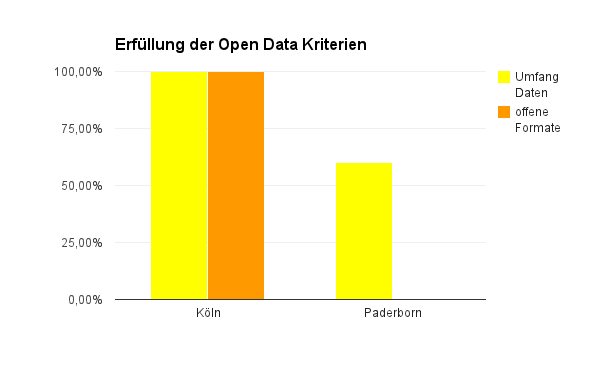
\includegraphics[scale=0.45]{section_paderborn_status.png}
 \end{figure}
 \begin{itemize}
  \item Paderborn \textbf{leicht} über Durchschnitt (49\%, 0,03\%)
  \item Keine Maschinenlesbaren Formate, aber relativ guter Datenumfang
 \end{itemize}
\end{frame}

\subsection{"Nicht-städtische" Daten}

\begin{frame}[t]{openstreetmap}
 \begin{figure}
  \centering
  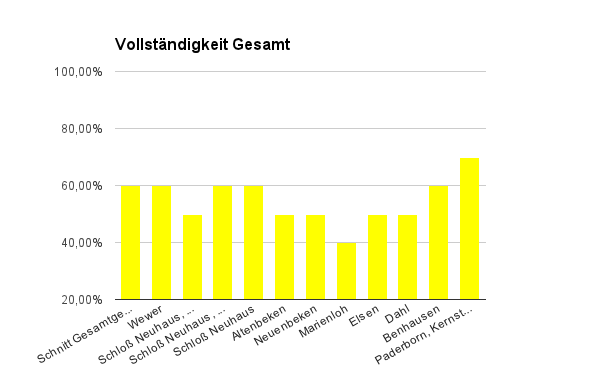
\includegraphics[scale=0.5]{section_paderborn_osm_overall.png}
 \end{figure}
\end{frame}


\begin{frame}[t]{openstreetmap 2}
 \begin{figure}
  \centering
  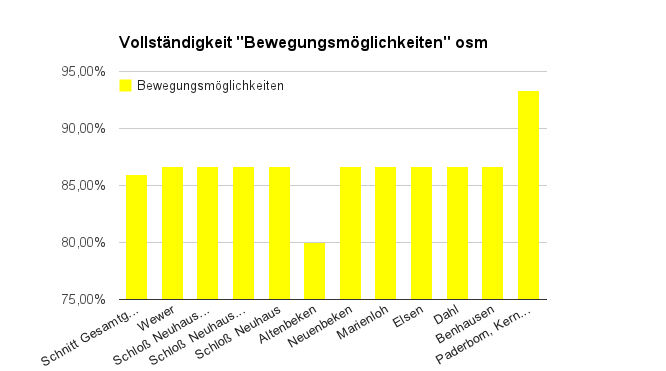
\includegraphics[scale=0.5]{section_paderborn_osm_move.png}
 \end{figure}
\end{frame}